\documentclass[10pt]{article}
\usepackage[utf8]{inputenc}
\usepackage{graphicx}
\begin{document}

\section*{Ejercicio 6}

Dada la siguiente distribución bidimensional:

\begin{center}
\begin{tabular}{c|cccc|c}
$X \backslash Y$ & 1 & 2 & 3 & 4 & $n_{i\cdot}$\\\hline
10 & 1 & 3 & 0 & 0 & 4 \\
12 & 0 & 1 & 4 & 3 & 8 \\
14 & 2 & 0 & 0 & 2 & 4 \\
16 & 4 & 0 & 0 & 0 & 4\\\hline
$n_{\cdot j}$ & 7 & 4 & 4 & 5 & 20\\
\end{tabular}
\end{center}

\begin{itemize}

\item[a)]¿Son estadísticamente independientes X e Y?

Se aprecia que $$n_{21} = 0 \not = \frac{n_{2\cdot}\cdot n_{\cdot 1}}{n} = \frac{56}{20},$$ por lo que no son independientes.

\item[b)]Calcular y representar las curvas de regresión de $X/Y$ e $Y/X$.

La curva de regresión de $Y$ sobre $X$ es $$(10,1'75), (12,3'25), (14,2'5), (16,1).$$

La curva de regresión de $X$ sobre $Y$ es  $$(14'5714,1), (10'5,2), (12,3), (12'8,4).$$

Representación:

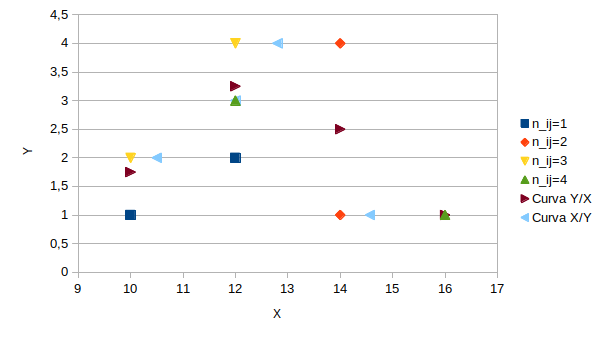
\includegraphics[width=10cm]{graficoe6.png}

\item[c)]Cuantificar el grado en que cada variable es explicada por la otra mediante la correspondiente curva de regresión.

Esto es cuantificado por la razón de correlación $\eta^2$: $$\eta^2_{Y/X} = \frac{\sigma^2_{ey}}{\sigma^2_y},$$ donde $\sigma^2_{ey}$ es la varianza explicada por la regresión $$\sigma^2_{ey} = \sigma^2_y - \sigma^2_{ry}$$ donde $\sigma^2_{ry}$ es la varianza residual $$\sigma^2_{ry} = \sum_{i=1}^k \sum_{j=1}^p f_{ij} [y_j - f(x_i)]^2$$ y $\sigma^2_y$ es la varianza de $Y$ $$\sigma^2_y = \mu_{02} = \sum_{j=1}^p f_{\cdot j}(y_j-\bar y)^2.$$
\\$\eta^2$ está entre 0 y 1; cuánto más cerca esté de 1 mejor ajustada está la correlación.

$$\bar y = 2,35$$

$$\sigma^2_y = 1,4275$$

$$\sigma^2_{ry} = 0,6625$$

$$\sigma^2_{ey} = 1,4275 - 0,6625 = 0,765$$

$$\eta^2_{Y/X} = \frac{0,765}{1,4275} = 0,5359$$

La variable $Y$ es parcialmente explicada por $X$ mediante la curva de regresión de $Y/X$.

$$\bar x = 12,8$$

$$\sigma^2_x = 4,16$$

$$\sigma^2_{ry} = 1,8757$$

$$\sigma^2_{ey} = 4,16 - 1,8757 = 2,2842$$

$$\eta^2_{X/Y} = \frac{2,2842}{4,16} = 0,5491$$

La variable $X$ es parcialmente explicada por $Y$ mediante la curva de regresión de $X/Y$.

\item[d)]¿Están $X$ e $Y$ correladas linealmente? Dar las expresiones de las rectas de regresión.

La correlación lineal se mide mediante el coeficiente de correlación lineal $r$:
$$r = \frac{\sigma_{xy}}{\sigma_x \sigma_y}$$
donde $\sigma_{xy}$ es la covarianza
$$\sigma_{xy} = \mu_{11} = m_{11} - \bar x \bar y$$
donde $m_{11}$ es el momento conjunto respecto al origen de órdenes 1 y 1,
$$m_{11} = \sum_{i=1}^k \sum_{j=1}^p f_{ij} x_i y_j,$$
$\sigma_x = +\sqrt{\sigma_x^2}$ es la desviación típica de $X$, y recíprocamente para $Y$.
\\$r$ está entre -1 y 1; cuánto más cerca esté de 0 menor es la correlación lineal.

$$m_{11} = 29,3$$
$$\sigma_{xy} = 29,3 - 12,8\cdot2,35 = -0,78$$
$$r = \frac{-0,78}{\sqrt{4,16}\sqrt{1,4275}} = -0,32008$$
La correlación lineal no explica bien la distribución.

En la recta de regresión $y = ax + b$, a es
$$a = \frac{\sigma_{xy}}{\sigma_x^2}$$
y b es
$$b = \bar y - \frac{\sigma_{xy}}{\sigma_x^2} \bar x.$$

Las expresiones de las rectas de regresión lineal son
$$y = -0,1875x + 4,75$$
y
$$x = -0,5464y + 14,08.$$

\end{itemize}

\end{document}